\documentclass[tikz,border=8pt]{standalone}
\usepackage{amsmath,amssymb}
\begin{document}
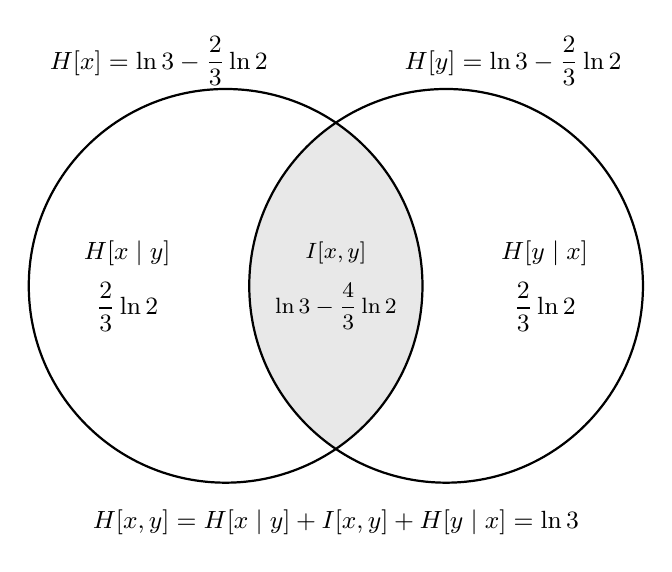
\begin{tikzpicture}[font=\small]
\begin{scope}
\clip (-1.4,0) circle (2.5);
\fill[gray!18] (1.4,0) circle (2.5);
\end{scope}
\draw[thick] (-1.4,0) circle (2.5);
\draw[thick] (1.4,0) circle (2.5);
\node[align=center] at (-2.65,0) {$H[x\mid y]$\\[5pt]$\dfrac23\ln2$};
\node[align=center,font=\footnotesize] at (0,0) {$I[x,y]$\\[6pt]$\ln3-\dfrac43\ln2$};
\node[align=center] at (2.65,0) {$H[y\mid x]$\\[5pt]$\dfrac23\ln2$};
\node at (-2.25,2.85) {$H[x]=\ln3-\dfrac23\ln2$};
\node at (2.25,2.85) {$H[y]=\ln3-\dfrac23\ln2$};
\node at (0,-3) {$H[x,y]=H[x\mid y]+I[x,y]+H[y\mid x]=\ln3$};
\end{tikzpicture}
\end{document}
